\documentclass[12pt]{article}
\usepackage{fontspec}
\usepackage{polyglossia}
\setdefaultlanguage{russian}
\setmainfont[Mapping=tex-text]{CMU Serif}
\usepackage{minted}
\newfontfamily{\cyrillicfonttt}[Scale=0.8]{Liberation Mono}
%\setdefaultlanguage{russian}
%\setmainfont[Mapping=tex-text]{CMU Serif}

\title{CEL MeshWorks}
\author{Владимир Петриго}
\date{Октябрь 2015}

\begin{document}

\maketitle

\section{Введение}

Стремительное развитие приборетает концепция Internet of Things (Интернет Вещей),
основной идеи которой является объединение бытовых и не только приборов или 
устройств в единую сеть. и производители очень часто предлагают различные 
средства для ускорения разработки либо для быстрой интеграции в 
\section{Аппаратная платформа MeshWorks}
\section{Скриптовый язык MeshWorks}

Модули, сенсорные узлы и ZigBee-интернет-шлюзы компании CEL имеют встроенную 
прошивку, которая позволяет интерпретировать инструкции скриптового языка 
MeshWorks. Синтаксис и форматирование данного языка схожи с языком Python. 
Пользователи могут использовать условные операторы if, tick-функции, вызываемые 
через заданный интервал времени, но специфических знаний в программировании не 
требуется. Основная задача данной платформы – упростить создание mesh-сети и 
работу устройств в ней.
Для написание и проверки скрипта компания CEL предлагает программное обеспечение 
MeshWorks GUI. Встроенные функции языка MeshWorks позволяют работать с периферией 
модуля, выполнять обработку, отправлять сетевые сообщения и т.д.
Ввиду того, что загружаемый в модули ZIC3588 скрипт интерпретируется встроенным 
программным обеспечением, это накладывает определенные ограничения на количество 
используемых элементов:
\begin{center}
\begin{tabular}{ |p{3cm}|p{2cm}|p{2cm}|p{2cm}|p{2cm}| } 
 \hline
 Тип & ZICM588SPx & ZICM357SPx & ZMW-SENSOR-1 & ZMW-GW-ETH-1 \\
 \hline
 Число отступов (табуляций) & 10 & 6 & 6 & 10 \\ 
 Tick-функции & 10 & 5 & 5 & 10 \\ 
 Числа & 9 & 7 & 7 & 9 \\ 
 Размер строки (символы) & 72 & 40 & 40 & 72 \\
 Размер строки (байтовое представление) & 36 & 20 & 20 & 36 \\
 Количество переменных & 251 & 91 & 91 & 251 \\
 Количество списков & 251 & 81 & 81 & 251 \\
 Размер скрипта (МБ) & 32 & 8 & 8 & 32 \\
 Количество символов в одной строке скрипта & 128 & 128 & 128 & 128 \\
 \hline
\end{tabular}
\end{center}
В таблице указаны максимальное количество элементов, которые интерпретатор MeshWorks может обработать.
\section{Особенности языка MeshWorks}
\subsection{Отступы}
Как и в языке Python, в MeshWorks для обозначения начала функции или условного 
выражения используется двоеточие «:». Кроме этого блоки кода определяются отступами. 
Увеличение отступа обозначает начало блока, а уменьшение – его конец. Если 
использовать GUI-интерфейс для написания скрипта, то нажатие клавиши Tab автоматически 
будет преобразовано в отступ в 4 пробельных символа. Если для написания скрипта 
используется стороннее программное обеспечение, то использование символов табуляции 
вместо пробелов является недопустимым. Поэтому рекомендуется перед отправкой скрипта 
на целевой узел открыть его в программе MeshWorks GUI для предварительного форматирования.
Пример написания функции с использованием языка MeshWorks:
\begin{minted}{python}
def function(number):
    print("Inside function)")
    
    if number == 1:
        print("Number = 1")
\end{minted}

\subsection{Комментарии}
Язык MeshWorks поддерживает строчные комментарии, которые начинаются со знака 
решетки «\#». Комментарий обязательно должен находиться на отдельной строке и 
может иметь дополнительные отступы.

Когда скрипт загружается в узел с прошивкой-интерпретатором MeshWorks, то все 
комментарии будут проигнорированы.
\begin{minted}{python}
def foo():
    # Комментарий
\end{minted}

Блочные комментарии не поддерживаются, но имеется возможность использовать 
несколько отдельных строк с предшествующим символом решетки:
\begin{minted}{python}
#-----------------
# Длинный комментарий
# Длинный комментарий
# Длинный комментарий
#-----------------
\end{minted}

\subsection{Переменные}
Для нужд программы пользователь может создавать собственные переменные. 
Идентификатор переменной должен начинаться с буквы (a-z,A-Z) может содержать 
латинские буквы (a-z,A-Z) и цифры (0-9).
Существуют также 3 переменные, которые пользователь должен инициализировать, так 
как они отвечают за название ZigBee-сети, имя устройства и возможность ухода в 
«спящий» режим.
\begin{minted}{python}
celPy.ApplicationName = "Your MeshWorks Network Name"
celPy.DeviceName = "Your MeshWorks Device Name"
celPy.IsSleepyDevice = True/False
\end{minted}
Переменная \textbf{ApplicationName} отвечает за имя сети. Для того, чтобы другие 
устройства могли подключиться к такой сети, необходимо задать аналогичное имя в 
каждом скрипте. Это имя служит для генерации ключа безопасноти, которое используется 
узлами в процессе подключения. Если необходимо иметь несколько различных сетей, 
то каждой сети необходимо дать свое имя.
Переменная \textbf{DeviceName} должна быть опредена либо с помощью ключевого 
слова «Gateway», которое задаст роль устройства как координатора, либо с помощью 
любого другого имени.
Переменная \textbf{IsSleepyDevice} определяет может ли устройство переходить в 
режим «сна» (True) либо нет (False).
\subsubsection{Работа с периферией}
Для работы с аппаратными возможностями модулей ZICM35XX MeshWorks использует так 
называемые Data Point (для представления входов) и Control Point (для представления 
выходов).\newline
Data Point представляет аппаратный вход микроконтроллера, который может быть цифровым 
или аналоговым входом или входом I2C-интерфейса. Например, такое представление 
может быть использовано для кнопки, аналогового или I2C-датчика.\newline
Control Point представляет аппаратный выход микроконтроллера, цифровой, аналоговый 
или I2C-выход. Например, вывод для управления светодиодом, аналоговый выход 
(ШИМ, динамик) или I2C-дисплей.
Data Point и Control Point объявляются в скрипте MeshWorks.\newline
Для создания Data Point необходимо задать имя, возможные состояния и интервал, 
с который аналоговое или цифровое значение вывода  будет считываться. Для Control 
Point проводится аналогичная процедура.\newline
Пример ниже показывает процесс создания Data Point для цифрового входа к которому 
подключена кнопка:
\begin{minted}{python}
# variable = [<name>, gpio, type, callback function, time in sec to call callback]
button = ["button", "PB6", "digital", "buttonF", 1]
# values = [type, number, first value, second value]
bValues = ["discrete", 2, "up", "down"]
\end{minted}
После того, как все Data и Control Point заданы их необходимо присвоить специльным 
переменным \textbf{celPy.DataCollectionPoints}, \textbf{celPy.DataCollectionValues},
\textbf{celPy.ControlPoints}, \textbf{celPy.ControlValues} как показано ниже:
\begin{minted}{python}
celPy.DataCollectionPoints = [button, reedSw,
tempSensor, humiditySensor, accel, proxSens]
celPy.DataCollectionValues = [bValues, rsValues,
tempSensorValues, humiditySensorValues, accelValues, proxValues]
celPy.ControlPoints = [greenLed, redLed, buzzer]
celPy.ControlValues = [greenValues, redValues, buzzerVal]
\end{minted}
\subsubsection{Целые числа}
Целые числа хранятся в 16-битных переменных (принимаемые значения -65535 – 65535). 
Значение переменным может быть присвоено с помощью шестнадцатеричной записи вида 0x0000 –
0xFFFF или с помощью чисел в десятичной системе 0 – 9. При записи шестнадцатеричных чисел
регистр букв (a-f A-F) не имеет значения, но префикс '0x' не может быть заменен на '0X'.
Значения, которые выходят за предел допустимых границ [-65535; 65535], будут 
принудительно усечены до значения максимального числа либо минимального, либо 
парсер выдаст предупреждение об ошибке.
Также поддерживаются булевы значения True (Истина) = 1 и False (Ложь) = 0.
Пример использования числовых переменных:
\begin{minted}{python}
celPy.ApplicationName = "networkName"
celPy.DeviceName = "Sensor"
celPy.IsSleepyDevice = False

# main
intMax = 0
#assign a value larger than allowed
intMax = 65535
#init integer to 0, subtract the desired negative number
intMin = 0
intMin = (intMin - 65535)
print("intMax = %d", intMax)
print("intMin = %d", intMin)
\end{minted}
\subsubsection{Строки}
Прошивка MeshWorks поддерживает ASCII-строки, которые могут содержать до 40 символов.
Содержимое строк ограничивается символом \". Допустимые символы: буквы в верхнем регистре A-Z,
буквы в нижнем регистре a-z, цифры 0-9, пробел и печатные ASCII-символы.
Кроме этого имеется возможность использования raw-строк, которые задаются 8-битным 
числом. Для использования необходимо перед началом строки поставить символ 'x'. 
Например, x"f005ba11" будет представлена на устройстве в виде последовательности 
байт 0xf0, 0x05, 0xba и 0x11.
Пример работы со строками:
\begin{minted}{python}
celPy.ApplicationName = "networkName"
celPy.DeviceName = "Sensor"
celPy.IsSleepyDevice = False

# main
def main():
    #longest ascii string
    asciiString = "The longest MeshWorks string is 40 chars."
    #longest byte string
    byteString = x"0102030405060708090A0B0C0D0F101112131415"
    print("asciiString = %s", asciiString)
    print("byteString = %s", byteString)
\end{minted}
\subsubsection{Поддержка подстановочных символов}
Очень часто возникает потребность отправки сообщений определенной группе устройств, 
которые имеют схожие имена (например «Light01», «Light02» и т.д.). Для таких 
целей в MeshWorks добавлена поддержка подстановочного символа «*» в функции 
\emph{celPy.AdjustRemoteControlPoint (имя устройства - строка, имя Control Point 
- строка, значение)} и \emph{celPy.setRemoteVariable (имя устройства - строка, 
имя переменной - строка, значение)}.
Например, имеется несколько узлов с именами \emph{Node01, Node02, Node03, Node04} 
и требуется на каждом узле выключить зеленый светодиод. Можно сделать так:
\begin{minted}{python}
celPy.AdjustRemoteControlPoint (Node01, greenLed, 0)
celPy.AdjustRemoteControlPoint (Node02, greenLed, 0)
celPy.AdjustRemoteControlPoint (Node03, greenLed, 0)
celPy.AdjustRemoteControlPoint (Node04, greenLed, 0)
\end{minted}
Но можно использовать подстановочный символ и сделать так:
\begin{minted}{python}
celPy.AdjustRemoteControlPoint (Node*, greenLed, 0)
\end{minted}
Тогда все узлы, имя которых начинается с «Node» получат данное сообщение. 
Либо если необходимо отправить широковещательную рассылку, можно использовать 
символ «*» следующим образом:
\begin{minted}{python}
celPy.AdjustRemoteControlPoint (*, greenLed, 0)
\end{minted}
\section{Функции}
\subsection{Типы функций}
В языке MeshWorks имеется три типа функций -- пользовательские функции, встроенные 
функции (например, для работы с периферией модуля) и глобальные функции 
(\emph{celPy.}-функции).\newline
\textbf{Пользовательские функции}\\
Для создания пользовательской функции используется ключевое слово \emph{def} 
за которым следует имя функции и в круглых скобках аргументы, которые функция 
принимает. После этого следует любое количество инструкций, которые функции выполняет.
Инструкции должны иметь хотя бы один 4-пробельный отступ.
Пример:
\begin{minted}{python}
def functionName(arg1, arg2, arg3):
    print("Inside function")
    if arg1 == 1:
        print("Inside function")
    else if arg2 == "hello":
        print("Inside function")

print("Not inside function")
\end{minted}
\textbf{Встроенные функции}\\
Встроенные функции предназначены для работы с периферией модуля. Они могут быть 
вызваны из функций, соответствующих Control или Data Point, так как это определяет
к каким вывода подключено то или иное устройство.\\
Функции работы с I2C:
\begin{minted}{python}
writeI2C(I2C address,
        byte value to write,
        register to write to)

Value = readI2C(I2C address,
                register to read from,
                keyword: littleEndian/bigEndian/singleByte,
                keyword: signed/unsigned)
\end{minted}
Функция \emph{writeI2C} отправляет один байт данных по указанному I2C-адресу и 
указанный регистр. Функция \emph{readI2C} предназначена для чтения информации с 
I2C-устройства 1 или 2 байт данных. Считывание только одного байта задается с 
помощью ключевого слова singleByte. Пользователь может задать порядок следования 
байтов (используя ключевое слове bigEndian или littleEndian). Последнее ключевое 
слово в функции \emph{readI2C} задает, как скрипт должен интерпретировать полученные 
значения -- как знаковое (signed) или беззнаковое (unsigned) значение.\\
Функции для работы с выводами:\\
\textbf{readDigital()}:
\begin{minted}{python}
# 1. button on PB6
button = ["button", "PB6", "digital", "buttonF", 1]
bValues = ["discrete", 2, "up", "down"]

def buttonF():
    # Read the digital value on pin PB6
    value = readDigital()
\end{minted}
Функция \emph{readDigital()} используется для того, чтобы считать состояние 
вывода порта модуля. В зависимости от текущего состояния возвращает либо 0, либо 1.\\
\textbf{readAnalog()}:
\begin{minted}{python}
# 3. Level Sensor (ADC) on PB5
lvlSens = ["lvlSens", "PB5", "analog", "lvlSensF", 1]
lvlSensValues = ["range", 0, 1, "volts"]
# Function to read level sensor
def lvlSensF():
    # Get ADC voltage on pin PB5 in 10ths of mV (0.1234V => 1234)
    value = readAnalog()
\end{minted}
Функция \emph{readAnalog()} возвращает аналоговое значение вывода в 16-разрядной 
переменной.\\
Функции для отправки сообщений на координатор \emph{sendDataReportString(string)}
и \emph{sendDataReport(numbericValue, label as String)}
\begin{minted}{python}
# read reed value
def reedSwF():
    value = readDigital()
    if (value == 1):
        sendDataReport("contact")
    if (value == 0):
        sendDataReport("no contact")
# function to read temperature
def tempMeasFunc():
    value = readI2c(0x41, 0xE3, bigEndian)
    # convert from reading to degrees C
    value = (value * 175)
    value = (value / 65535)
    value = (value - 47)
    # convert from degrees C to degrees F
    value = (value * 18)
    value = (value / 10)
    value = (value + 32)
    sendDataReport(value, "degrees F")
\end{minted}
При вызове этих функции на координатор отправляется соответствующая информация 
об адресе узла, имя Data Point и переданные значения.\\
\textbf{Встроенные глобальные функции}\\
Функция \emph{celPy.AdjustLocalControlPoint(ControlPointName – строка, NewValue 
– строка или число)} позволяет установить значение в соответствующем Control Point.
Например:
\begin{minted}{python}
# turn on local LED (LED is active low)
celPy.AdjustLocalControlPoint("greenLed", 0)
# turn off local LED (LED is active low)
celPy.AdjustLocalControlPoint("greenLed", 1)
\end{minted}
\subsection{Периодические функции}
Добавление периодических функций позволяет совершать какое-то действие через 
определенный интервал времени. Эту возможность предоставляет глобальная функция 
\emph{celPy.addTickFunction(functionName, N)}. В качестве аргумента functionName 
передается имя созданной пользовательской функции, а аргумент N отвечает за 
интервал времени, через который эта функция будет вызываться. N - число 100 мс 
интервалов, которые пройдут прежде чем будет вызвана функция functionName.
Для примера, мы передали N = 50. Следовательно, функция будет вызваться каждые 
50 * 100 мс = 5000 мс = 5 с. \\
Пример использования:
\begin{minted}{python}
# blink the LED every 2 second
celPy.addTickFunction(heartbeatLed, 20)

ledState = 0

def heartbeatLed():
    if (ledState == 0):
        celPy.AdjustLocalControlPoint("greenLed", 1)
        ledState = 1
        # return added for not being handled by second if
        # statement
        return
    if (ledState == 1):
        celPy.AdjustLocalControlPoint("greenLed", 0)
        ledState = 0
\end{minted}
\subsection{Управление удаленными узлами}
В MeshWorks встроена фукнция, позволяющая управлять состояниями на удаленных узлах.
Для этого используется функция:
\begin{minted}{python}
celPy.AdjustRemoteControlPoint("receivingDeviceName", 
                                "variableName", variableValue)
\end{minted}
, где receivingDeviceName - строка с именем устройства, variableName - строка с 
именем переменной, variableValue - значение, которое необходимо установить (может 
быть как строкой, так и числом). Для того чтобы использовать возможности функции 
\emph{celPy.AdjustRemoteControlPoint}, необходимо чтобы на принимающем узле была 
реализована функция \emph{cpCallbackVariableUpdate}. Эта функция будет автоматически 
вызываться, когда придет запрос на изменение значение от удаленного узла.
Например, один узел отправляет команду на включение лампочки:
\begin{minted}{python}
celPy.setRemoteVariable("Light01", "on/off", 1)
\end{minted}
На принимающем узле «Light01» функция \emph{cpCallbackVariableUpdate} должна быть
реализована так:
\begin{minted}{python}
def cpCallbackVariableUpdate(variableName, value):
    if (variableName == "on/off"):
        celPy.AdjustLocalControlPoint("greenLed", value)
\end{minted}
\subsection{Функции для работы со строками}
Для удобства разработчиков MeshWorks имеет ряд функций, позволяющих выполнять 
преобразование строк:
\begin{itemize}
    \item Функция, возвращающая целочисленной значение переданной строки по заданному
основанию base = (10, 16)\\
        \begin{minted}{python}
        string.atoi(string, base)
        # Пример
        str1 = "123"
        str2 = "a"
        val1 = string.atoi(str1, 10) # val1 = 123
        val1 = string.atoi(str1, 16) # val1 = 10
        \end{minted}
    \item Функция, возвращающая подстроку. Начало подстроки - stratIndex, конец - 
endIndex\\
        \begin{minted}{python}
        string.substring(string, startIndex, endIndex)
        # Пример
        str3 = "abcdefghi"
        str4 = string.substring(str3, 0, 2)
        print("str4 %s", str4)
        # str4 abc
        str4 = string.substring(str3, 3, 5)
        print("str4 %s", str4)
        # str4 def
        str4 = string.substring(str3, 6, 8)
        print("str4 %s", str4)
        # str4 ghi
        \end{minted}
    \item Функция для поиска первого вхождения в строку string to search строки
string to find. Если строка найдена возвращается индекс вхождения, в противном 
случае возвращается 255:
        \begin{minted}{python}
        string.find(string to search, string to find)
        # Пример
        str3 = "abcdefghi"
        find1 = string.find(str3, "bc")
        print("find1 %d", find1)
        # find1 = 1
        \end{minted}
\end{itemize}
\subsection{Работа с Ethernet-функциями}
Для организации взаимодействия сетей MeshWorks с локальной или глобальной сетью
прошивка-интерпретатор ZigBee-Ethernet-шлюзов поддерживает набор функций, которые
позволяют организовать отправку TCP/UDP/HTTP-сообщений.

Также имеется возможность получения входящих сообщений, которые обрабатываются в
callback-функциях для соответствующего транспортного протокола.

Функции для организации отправки сообщений:
    \begin{minted}{python}
    tcp.send(destination, port, tcpPayloadString)
    udp.send(destination, port, udpPayloadString)
    http.send(destination, httpPayload)
    \end{minted}

, где \emph{destination} - может быть IP-адресом или URL-ссылкой, \emph{port} 
(для TCP и UDP-сообщений) - порт, который прослушивает стороннее приложение, 
\emph{payload} - сообщение для отправки.

Для приема TCP и HTTP-пакетов есть две соответствующие callback-функции, которые
будут вызваны при получении соответствующего сообщения.
    \begin{minted}{python}
    cpCallbackTcpReceived(type, ip, srcPort, dstPort, data)
    cpCallbackHttpReceived(type, ip, srcPort, dstPort, data)
    \end{minted}
    
, где \emph{ip} - IP-адрес отправителя, \emph{srcPort} - порт отправителя, 
\emph{dstPort} - порт назначения, \emph{data} - данные.

Пример использования функции отправки TCP-сообщения на шлюзе ZMW-GW-ETH-1:
    \begin{minted}{python}
    # кнопка на GPIO PA3 
    buttonPoint = ["button", "PA3", "digital", "buttonF", 1]
    buttonValues = ["discrete", 2, "up", "down"]
    # Конфигурация узла
    celPy.ApplicationName = "MeshWorks"   
    celPy.DeviceName = "Gateway"
    celPy.IsSleepyDevice = False
    celPy.DataCollectionPoints = [buttonPoint]  
    celPy.DataCollectionValues = [buttonValues] 
    
    # строки для передачи состояния кнопки
    pr = "pressed"
    rel = "released"

    def buttonF():
        value = readDigital()
        # кнопка нажата
        if (value == 1):
            tcp.send("192.168.0.1", 5005, pr)
            return
        # кнопка отпущена
        if (value == 0):
            tcp.send("192.168.0.1", 5005, rel)

    # Стартовая main() функция   
    def main(): 
        # Отправка информации на сервер о начале работы шлюза
        tcp.send("192.168.0.1", 5005, "READY")
    \end{minted}
\subsection{Контроль портов ввода/вывода в различных режимах работы}
Функции контроля портов ввода/вывода позволяют настроить состояние и направление
определенного вывода, когда узел находится в спящем или активном режиме.
Это позволяет оптимизировать энергопотребление узла в различных режимах работы.
Общая рекомендация при использовании спящих узлов --- на время сна переводить все
неиспользуемые выводы в режим входа с подтяжкой.
    \begin{itemize}
    \item \emph{celPy.setPinSleepState(pin name, cfgPowerDown, gpioOutPowerDown)}
    - задание конфигурации вывода модуля при нахождении в спящем режиме (например, 
    переключение на вход с использованием подтягивающего резистора)
    \item \emph{celPy.setPinWakeState(pin name, cfgPowerDown, gpioOutPowerDown)}
    - задание конфигурации вывода модуля при нахождении в активном режиме (например,
    аналоговый вход)
    \end{itemize}

Возможные значения аргумента \textit{\textbf{cfgPowerDown}}:
    \begin{itemize}
    \item \textbf{OUT} - выход
    \item \textbf{OUT_OD} - выход open-drain (открытый коллектор)
    \item \textbf{OUT_ALT} - выход, альтернативная функция 
    \item \textbf{OUT_ALT_OD} - выход, альтернативная функция в режиме «открытый коллектор» (например линия I2C)
    \item \textbf{ANALOG} - аналоговый вход/выход
    \item \textbf{IN} - вход (float)
    \item \textbf{IN_PUD} - вход с поддтяжкой
    \end{itemize}
    
Возможные значения аргумента \textit{\textbf{gpioOutPowerDown}}:
    \begin{itemize}
    \item \textbf{PULLUP} -- подтяжка к напряжению питания «1»
    \item \textbf{PULLDOWN} -- подтяжка к уровню земли «0»
    \end{itemize}

Пример использования:
    \begin{minted}{python}
        celPy.setPinSleepState("PA0", "ANALOG", "PULLDOWN")
        celPy.setPinWakeState("PA6", "OUT", "PULLUP")
    \end{minted}
    
\section{Математические и условные операторы}
\subsection{Математические операторы}
Чтобы иметь возможность делать предварительную обработку данных поступающих 
с аналоговых входов, работать со счетчиками либо реализовывать какую-либо другую
доступную логику работы в языке MeshWorks поддерживаются основные математические 
операторы для работы с целыми числами (во всех примерах res = 0, a = 10, b = 20):
\begin{table}[h!}
\centering
    \begin{tabular}{|c|c|c|}
    \hline
    Оператор & Описание & Пример\\
    \hline
    + & Сложение & res = a + b; res = 30\\
    \hline
    - & Вычитание & res = a - b; res = -10\\
    \hline
    * & Умножение & res = a * b; res = 200\\
    \hline
    / & Деление & res = a / b; res = 0\\
    \hline
    \end{tabular}
\end{table}
\subsection{Условный оператор if}
Условный оператор \textbf{if} предназначен для организации ветвлений в логике 
программы. Для использования условий необходимо указать ключевое слово \emph{if},
затем в круглых скобках условие и поставить двоеточие в конце.
\begin{minted}{python}
    if (A operator B) :
        # обработка в случае,
        # если условие верно
        
        # выход из функции
        return
    # если нет то будет выполнен
    # код ниже
\end{minted}

A и B могут быть переменными, числами или строками. Вместо \emph{operator} должен
стоят оператор равенства или неравенства. Если выражение (A operator B) принимает
значение истины (True), тогда код внутри условного оператора будет выполнен, в противном
случае, если условие (A operator B) ложно (False) выполнение продолжится сразу за
блоком if.

В таблице ниже указаны все доступные операторы (для примера arg1 = 1, arg 2 = 2):
\begin{table}[h!}
\centering
    \begin{tabular}{|c|c|c|}
    \hline
    Оператор & Описание & Пример\\
    \hline
    == & Равенство & (arg1 == arg2) -> False\\
    \hline
    != & Неравенство & (arg1 != arg2) -> True\\
    \hline
    > & Больше, чем & (arg1 > arg2) -> False\\
    \hline
    < & Меньше, чем & (arg1 < arg2) -> True\\
    \hline
    \end{tabular}
\end{table}

Так как в MeshWorks нет поддержки конструкции if-else, то для того, чтобы избежать
ложного входа в другие условыне операторы, необходимо использовать ключевое слово
\emph{return}:
\begin{minted}{python}
# установка tick-функции с интервалом в 2 секунды
celPy.addTickFunction(heartbeatLed, 20)

# первоначальная инициализация
ledState = 0
# инвертирование состояния светодиода
def heartbeatLed():
    if (ledState == 0):
    celPy.AdjustLocalControlPoint("greenLed", 1)
    ledState = 1
    # выход из функции с помощью return
    # если его не сделать, то выполнение 
    # функции продолжится и программа
    # попадет в следующий условный оператор
    return
    if (ledState == 1):
    celPy.AdjustLocalControlPoint("greenLed", 0)
    ledState = 0
\end{minted}
\section{Пример работы}
В качестве демонстрационного примера решим следующую задачу. Имеется две комнаты,
температуру в которых необходимо измерить, а также есть два выключателя, которые
должны управлять состоянием лампочек. И все данные о температуре и состоянии
выключателей должны передаваться на централизованный сервер. Примерная структурная
схема представлена на рисунке 1.
\begin{figure}[h!]
    \centering
    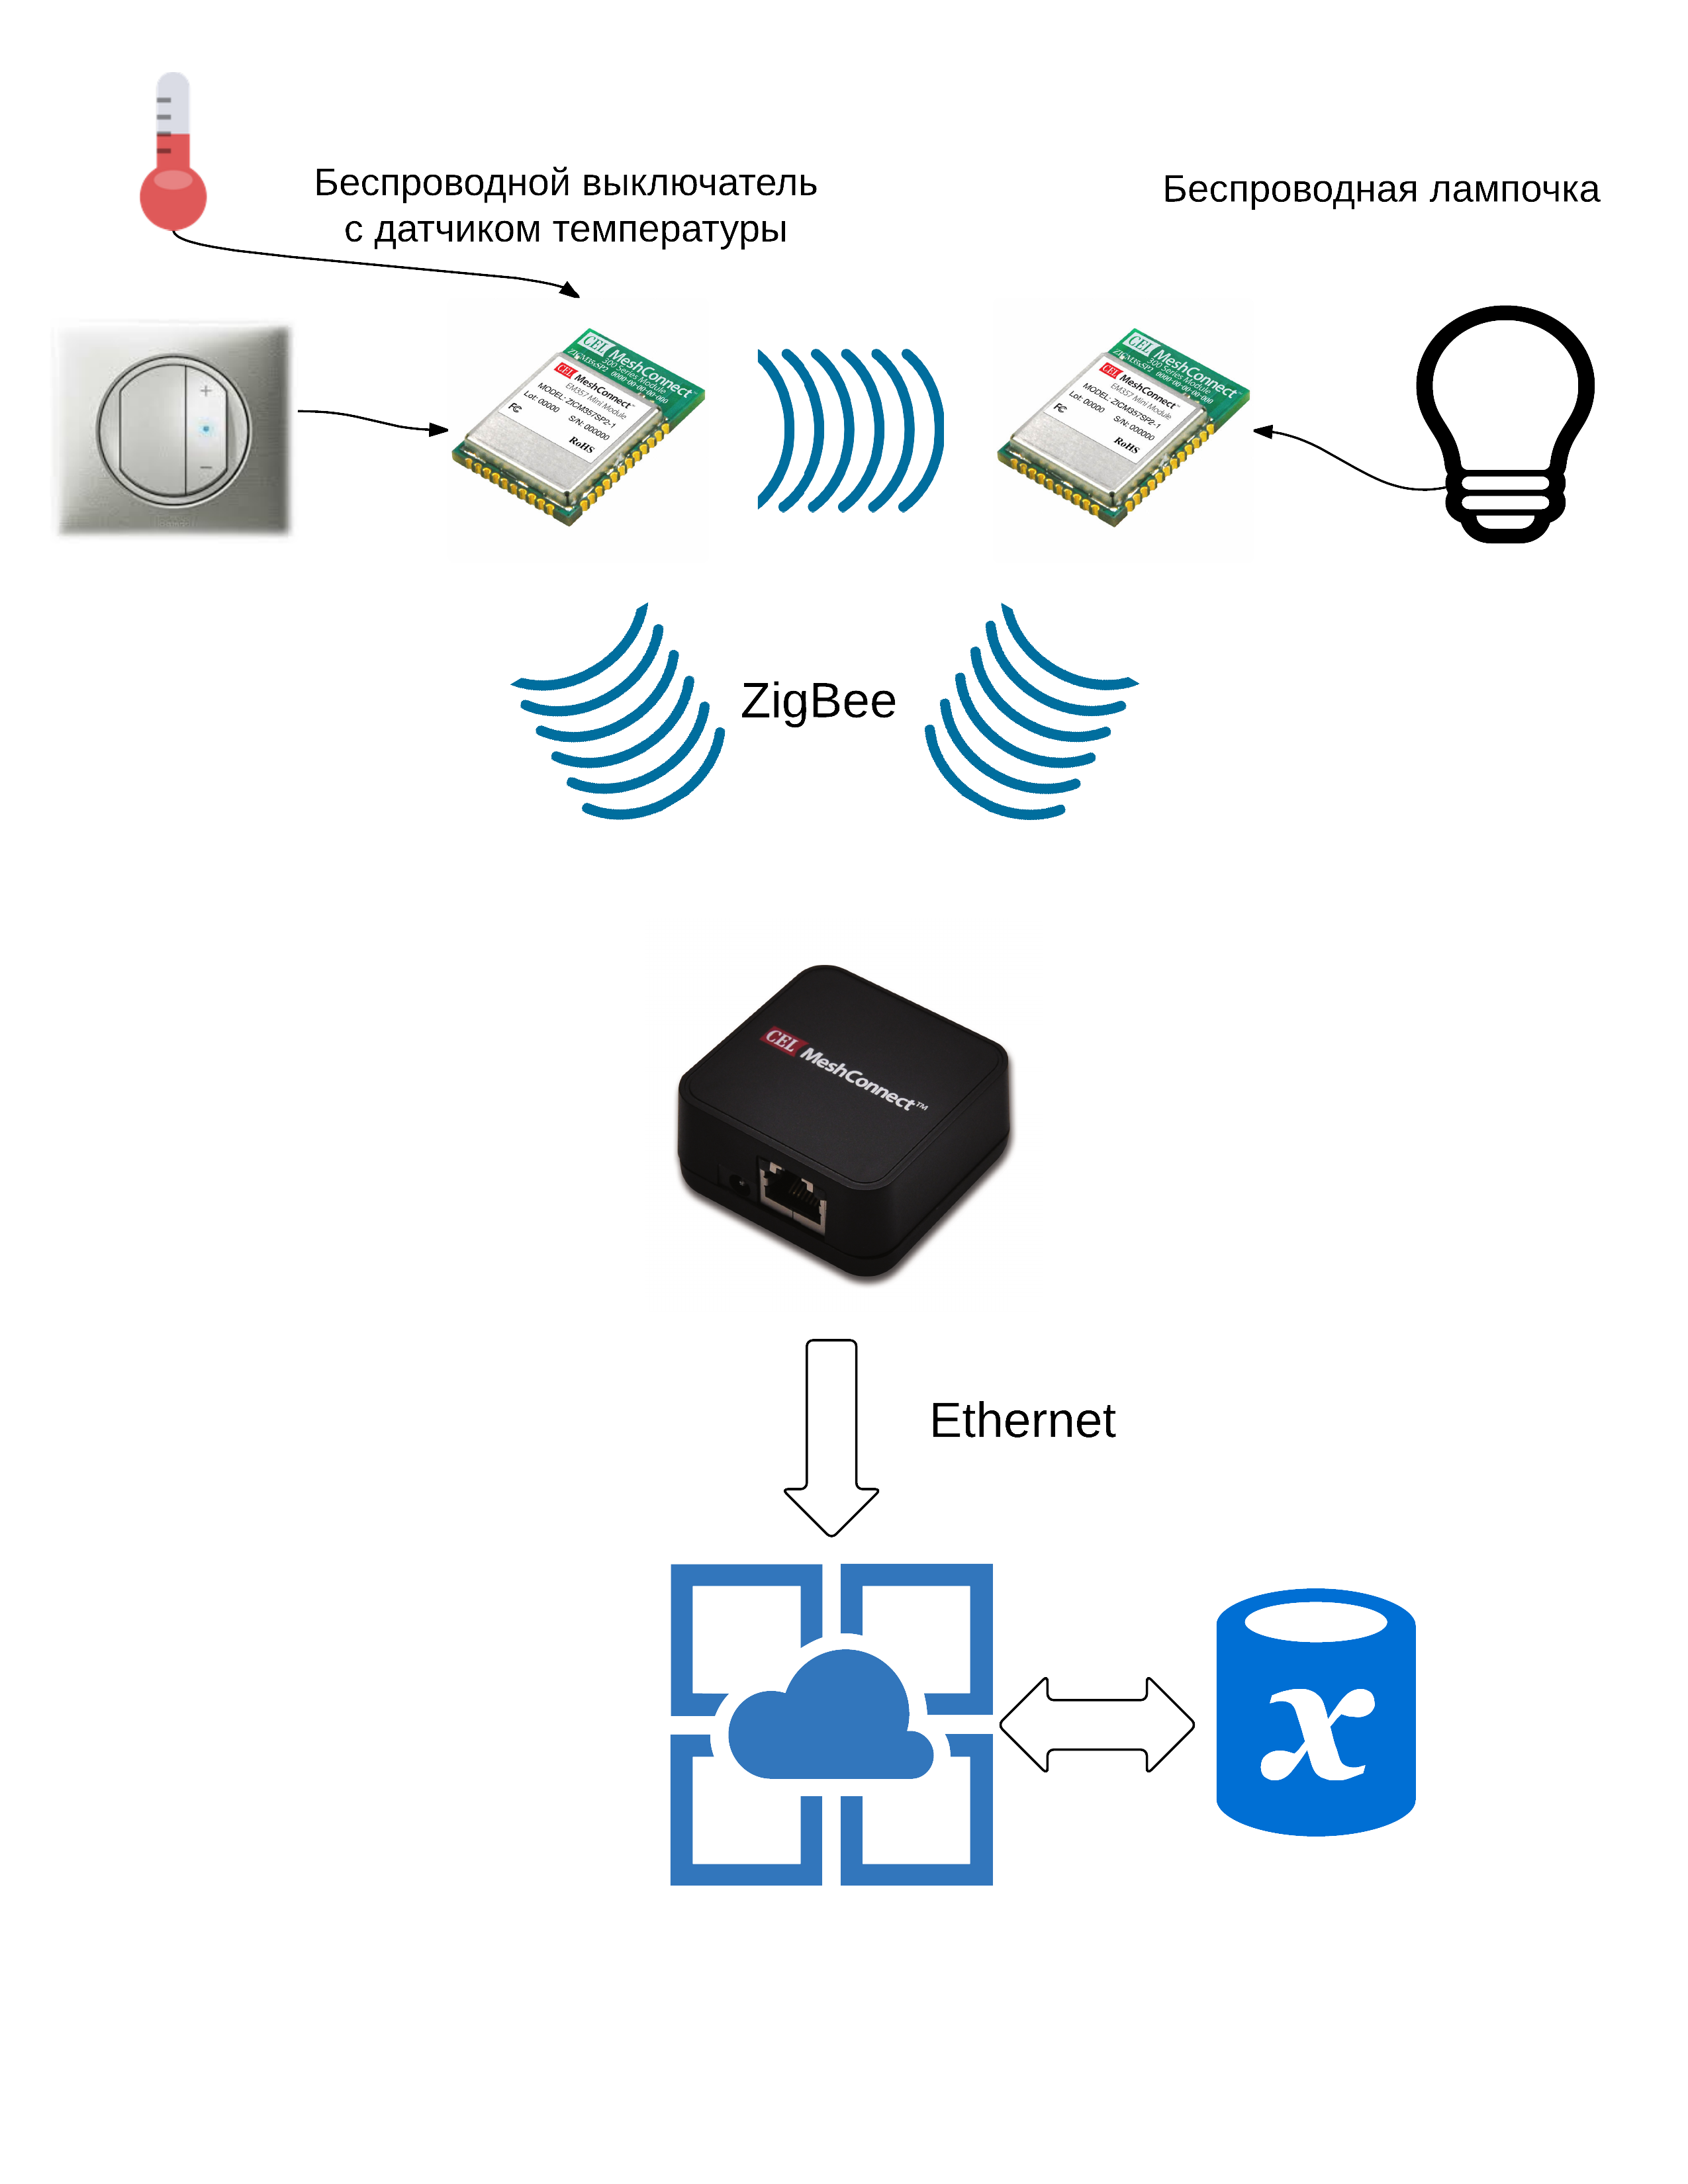
\includegraphics[scale=0.5]{cel-structure.png}
    \caption{Структурная схема примера}
\end{figure}

Выключатель, ламочка подключены к цифровым входам модуля CEL ZICM3588, в качестве
датчика температуры используется однокристальный датчик влажности и температуры
Si7013 с I2C-интерфейсом.

При изменении состояния выключателя лампочка включается или выключается. Также 1 раз в 20
секунд обновляется информация о значении температуры в комнате. Информацию об этом
каждый узел передает по радиоканалу на центральный шлюз. Центральный шлюз всю
полученную информацию передает на локальный или глобальный сервер.

\section{Заключение}

\end{document}
